\section[Gradient]{A learning paradigm for interpretable gradients}
%--------------------------------------------------------------------------------------------------
\begin{frame}[t]
    \frametitle{Preliminaries}
    \framesubtitle{Premise}
    \begin{center}
        \emph{Gradient information is noisy and hard to interpret, 
        however smoothing it makes it discriminative. Can gradient
         information be denoised during training, improving interpretability properties? }
        \vspace{20pt}
        \begin{columns}
            \column{0.2\textwidth}
            \column{0.4\textwidth}
                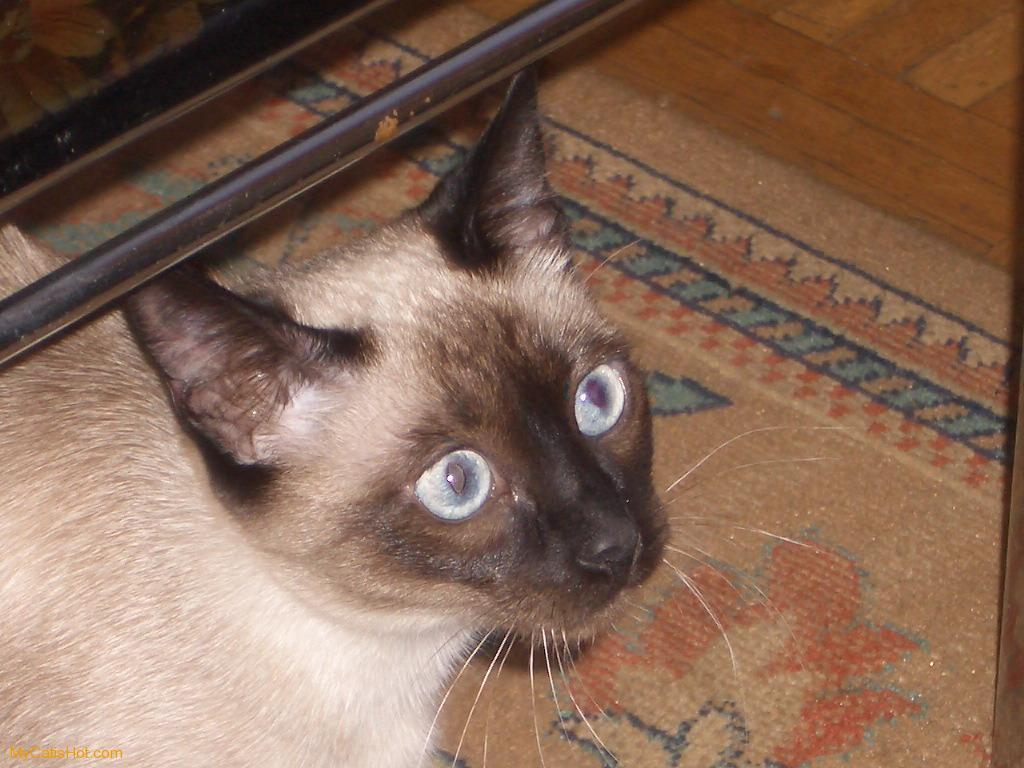
\includegraphics[width=0.95\textwidth]{fig/gradient/fig/method/input.jpg}
            \column{0.2\textwidth}
                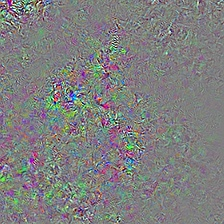
\includegraphics[width=0.95\textwidth]{fig/gradient/fig/method/gradient.jpg}\\
                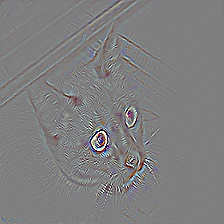
\includegraphics[width=0.95\textwidth]{fig/gradient/fig/method/guided_gradient.jpg}
            \column{0.2\textwidth}

        \end{columns}
        %\input{fig/castream/tex/ca_mainfig.tex}
    \end{center}
\end{frame}
%--------------------------------------------------------------------------------------------------
\begin{frame}
    \frametitle{Preliminaries}
    \framesubtitle{Contributions}
    \begin{itemize}
        \item Novel regularization for interpretable guided training.
        \item Improvement of post-hoc interpretations following transparency ideas.
         
    \end{itemize}
    %\begin{itemize}
        %\item \textbf{CAM is Attention}\\
        %We demonstrate that CAM behaves in a similar manner as attention.
        %\item \textbf{Cross Attention: [CLS] on CNNs}\\
        %We train an abstract class representation using a stream, alongside standard CNNs.
        %\item \textbf{CAM on more architectures}\\
        %CAM is usually validated only on ResNet and VGG. Extension to ConvNeXt.
    %\end{itemize}
\end{frame}
%--------------------------------------------------------------------------------------------------
\subsection*{Motivation}
%--------------------------------------------------------------------------------------------------
\begin{frame}[t]
    \frametitle{Interpretable Gradients}
    \framesubtitle{Leveraging Backpropagation}
    \small 
    The response ($y$) of a model ($f$) parameters ($\phi$) , after forwarding an input $x$ can be 
    visualized on the input space, via backpropagation:
    \begin{equation}
        \frac{\partial x}{\partial y} = \frac{\partial x}{\partial F_0}\frac{\partial F_0}{\partial F_1}\cdot\dots\cdot\frac
        {\partial F_{-1}}{\partial y}
        \label{eq:backtoin}
    \end{equation}
    \pause
    However, due to non-linearities it is noisy:
    \begin{columns}
        \column{.2\textwidth}
        \column{.3\textwidth}
            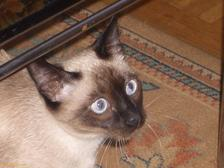
\includegraphics[width=.95\textwidth]{fig/gradient/fig/Original_Input.JPEG}
        \column{.3\textwidth}
            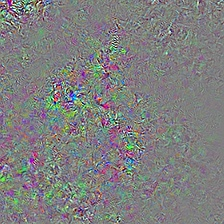
\includegraphics[width=.95\textwidth]{fig/gradient/fig/method/gradient.jpg}
        \column{.2\textwidth}
    \end{columns}
\end{frame}
%--------------------------------------------------------------------------------------------------
\begin{frame}[t]
    \frametitle{Interpretable Gradients}
    \framesubtitle{Soft Gradients}
    \small
    Soft gradients can be achieved by two approaches:
    \begin{columns}
        \footnotesize
        \column[T]{.5\textwidth}
            \textbf{Guided Backpropagation \cite{guidedbackprop}}\\
            Achieved by constraining backprop to only let 
            positive gradients flow:
            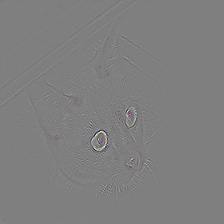
\includegraphics[width=.80\textwidth]{fig/gradient/fig/gb_standard.jpg}
            \pause
        \column[T]{.5\textwidth}
            \textbf{Smoothgrad \cite{smilkov2017smoothgrad}}\\
            Achieved by iteratively adding noise to the input space prior to forward pass:
            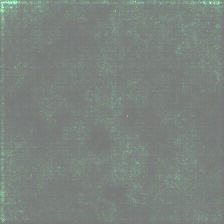
\includegraphics[width=.80\textwidth]{fig/gradient/fig/gb_smooth.jpg}
    \end{columns}
\end{frame}
\subsection*{Method}
%--------------------------------------------------------------------------------------------------
\begin{frame}[c]
    \frametitle{Interpretable Gradients}    
    \framesubtitle{Formalized}
    \small
    Goal: Denoise the gradient during training using guided backprop.\\
    \emph{How?} Regularize using guided backprop.\\\pause
    \resizebox{\textwidth}{!}{
	\begin{tikzpicture}[
		scale=.3,
		font={\footnotesize},
		node distance=.5,
		label distance=3pt,
		wide/.style={yscale=.75},
		net/.style={draw,trapezium,trapezium angle=75,inner sep=3pt},
		enc/.style={net,shape border rotate=270},
		dec/.style={net,shape border rotate=90},
		txt/.style={inner sep=3pt},
		loose/.style={looseness=.6},
		sg/.style={blue!60},
	]
	\matrix[
		tight,row sep=6,column sep=16,
		cells={scale=.3,},
	] {
		\&\&\&\&\&
		\node[dec] (guided-back) {guided \\ backprop}; \&
		\node[wide,label=90:$\ipder{_G L_C}{x}$] (guided) {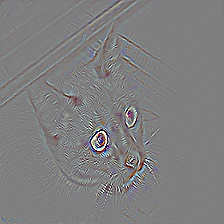
\includegraphics[width=.25\textwidth]{fig/gradient/fig/method/guided_gradient.jpg}}; \\
		\node[label=90:input image $x$] (in) {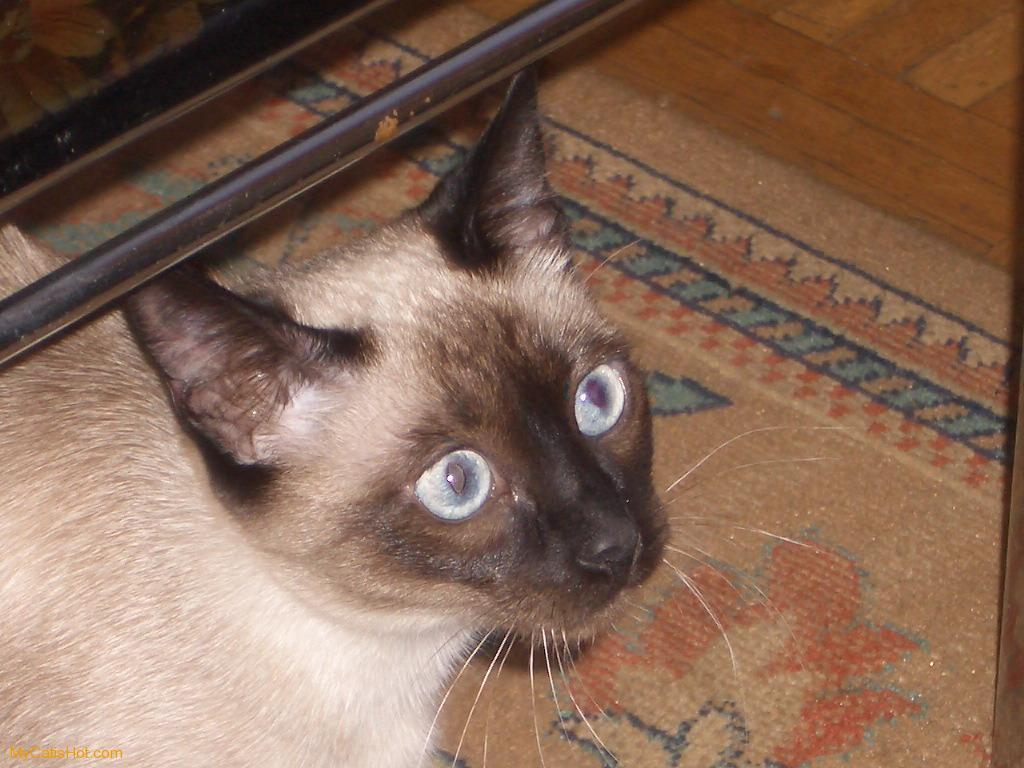
\includegraphics[width=.25\textwidth]{fig/gradient/fig/method/input.jpg}}; \&
		\node[enc] (net) {network \\ $f$}; \&\&\&
		\node[box] (class) {classification \\ loss $L_C$}; \&
		\node[dec] (back) {standard \\ backprop}; \&
		\node[wide,label=90:$\ipder{L_C}{x}$] (grad) {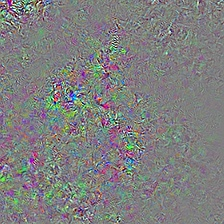
\includegraphics[width=.25\textwidth]{fig/gradient/fig/method/gradient.jpg}}; \&
		\node[box] (reg) {regularization \\ loss $L_R$}; \\
		\&\&\&\&\&\&\&
		\node[op] (plus) {$+$}; \&
		\node[txt] (loss) {total loss \\ $L = L_C + $\\ $\lambda L_R$}; \\
	};

	\draw[->]
		(in) edge (net)
		(net) edge node[above] {logits $y$} (class)
		(class) edge (back)
		(back) edge (grad)
		(guided-back) edge[sg] (guided)
		(grad) edge (reg)
		(reg) edge (plus)
		(plus) edge (loss)
		(class) edge[sg,out=90,in=180] (guided-back)
		(class) edge[loose,out=-50,in=180] (plus)
		(guided) edge[sg,out=0,in=90] node[pos=.2,font=\large,label=0:stop gradient] {//} (reg)
		(net) edge[dashed,out=60,in=150] (guided-back)
		(net) edge[dashed,out=30,in=150] (back)
		;
	\end{tikzpicture}
}
\end{frame}
%--------------------------------------------------------------------------------------------------
\begin{frame}[t]
    \frametitle{Interpretable Gradients}
    \framesubtitle{Smooth Gradient as Regularization}
    \small
    Assuming target labels $T$:
    \begin{equation}
        L_R(X, \theta, T) = \frac{1}{n} \sum_{i=1}^n E(\delta x_i, \delta_G x_i),
    \end{equation}
    \pause
    And the total loss:
    \begin{equation}
        L(x, \theta, t) = L_C(x, \theta, t) + \lambda L_R(x, \theta, t),
    \label{eq:total}
    \end{equation}
\end{frame}
%--------------------------------------------------------------------------------------------------

%--------------------------------------------------------------------------------------------------
\subsection*{Set-Up}
\begin{frame}[t]
    \frametitle{Experimental Set-Up}
    {\footnotesize
    \begin{columns}
        \column[T]{.5\textwidth}
        \textbf{Training and models}
            \begin{itemize}
                \item Training and validation in train and val sets of CIFAR-100
                (\cite{krizhevsky2009learning}) respectively.
                \item Using an optimized recipe for the dataset  \footnotemark.
                % (90 epochs, SGD optimization \cite{bottou2010large}, 
                % lr decay every 90 epochs).\footnotemark
                \item Training ResNet (18), MobileNet \cite{DBLP:journals/corr/HowardZCKWWAA17}.
                %Finetuning from ImageNet models.
                

            \end{itemize}\pause
        \column[T]{.5\textwidth}
        \textbf{Evaluation }
        \begin{itemize}
            \item CIFAR has no center crop. All image it is.%.
            \item No localization evaluation.%, lessons learnt from Opti-CAM.
            %\item Raw Attention used for OOD data.%, highlights on unseen data.
            \item Ablation on regularization functions.
        \end{itemize}
    \end{columns}
    }
    \footnotetext{\tiny{\url{https://github.com/weiaicunzai/pytorch-cifar100}}}
    %\footnotetext[2]{\tiny{{Timm \url{https://github.com/rwightman/pytorch-image-models}}}}
    %\footnote{https://github.com/weiaicunzai/pytorch-cifar100}
\end{frame}
\subsection*{Experiments}
%--------------------------------------------------------------------------------------------------
%\begin{frame}[t]
%    \frametitle{Results}
%    \framesubtitle{Qualitative Experiments}
%    \small
%    \textbf{Denoising effect}
%    \begin{center}
%        %\begin{figure}[H]
%    \scriptsize
%    \centering
    \setlength{\tabcolsep}{1.5pt}
    \begin{tabular}{cccccc}
        &\footnotesize Bed &\footnotesize Lamp &\footnotesize Lawnmower &\footnotesize Maple Tree &\footnotesize Sunflower\\
        {\rotatebox{90}{\Th{Input}}}&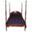
\includegraphics[width=.15\textwidth]{fig/gradient/fig/fig_grad/original/5415.JPEG} &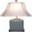
\includegraphics[width=.15\textwidth]{fig/gradient/fig/fig_grad/original/1766.JPEG} &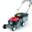
\includegraphics[width=.15\textwidth]{fig/gradient/fig/fig_grad/original/8311.JPEG} &
        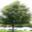
\includegraphics[width=.15\textwidth]{fig/gradient/fig/fig_grad/original/1198.JPEG} & 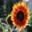
\includegraphics[width=.15\textwidth]{fig/gradient/fig/fig_grad/original/8881.JPEG}\\

        {\rotatebox{90}{\Th{Baseline}}}&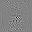
\includegraphics[width=.15\textwidth]{fig/gradient/fig/fig_grad/baseline/5415.JPEG} &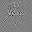
\includegraphics[width=.15\textwidth]{fig/gradient/fig/fig_grad/baseline/1766.JPEG} &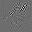
\includegraphics[width=.15\textwidth]{fig/gradient/fig/fig_grad/baseline/8311.JPEG} &
        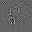
\includegraphics[width=.15\textwidth]{fig/gradient/fig/fig_grad/baseline/1198.JPEG} & 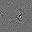
\includegraphics[width=.15\textwidth]{fig/gradient/fig/fig_grad/baseline/8881.JPEG}\\

        {\rotatebox{90}{\Th{Ours}}}&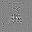
\includegraphics[width=.15\textwidth]{fig/gradient/fig/fig_grad/cosine/5415.JPEG} &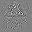
\includegraphics[width=.15\textwidth]{fig/gradient/fig/fig_grad/cosine/1766.JPEG} &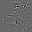
\includegraphics[width=.15\textwidth]{fig/gradient/fig/fig_grad/cosine/8311.JPEG} &
        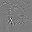
\includegraphics[width=.15\textwidth]{fig/gradient/fig/fig_grad/cosine/1198.JPEG} & 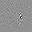
\includegraphics[width=.15\textwidth]{fig/gradient/fig/fig_grad/cosine/8881.JPEG}\\

    \end{tabular}
%    \caption{\textbf{Gradient comparison} of standard \vs our training on CIFAR-100 examples.}
%    \label{fig:grads}
%    \end{figure}
%    \end{center}
%    
%\end{frame}
%--------------------------------------------------------------------------------------------------
\begin{frame}[t]
    \frametitle{Results}
    \framesubtitle{Qualitative Experiments}
    \small
    \textbf{CAM  Visualizations}
    \begin{center}
        %\begin{figure}[H]
%    \tiny
%    \centering
%\resizebox{\textwidth}{!}{%}}
    \setlength{\tabcolsep}{.25pt}
    \begin{tabular}{cccccccccc}
        & \mr{2}{\tiny\Th{Input}} & \mc{2}{\tiny\Th{Grad-CAM}} & \mc{2}{\tiny\Th{Grad-CAM++}} & \mc{2}{\tiny\Th{Score-CAM}} & \mc{2}{\tiny\Th{Ablation-CAM}} \\
        & & \tiny\Th{Baseline} & \tiny\Th{Ours} & \tiny\Th{Baseline} & \tiny\Th{Ours} & \tiny\Th{Baseline} & \tiny\Th{Ours} & \tiny\Th{Baseline} & \tiny\Th{Ours} \\
    
         {\rotatebox{90}{\tiny \Th{Man}}} &
         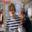
\includegraphics[width=.09\textwidth]{fig/gradient/fig/fig_cam/original/4862.JPEG} &
         \includegraphics[width=.09\textwidth]{fig/gradient/fig/fig_cam/baseline/gradcam/4862.JPEG} &
         \includegraphics[width=.09\textwidth]{fig/gradient/fig/fig_cam/cosine/gradcam/4862.JPEG} &
         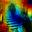
\includegraphics[width=.09\textwidth]{fig/gradient/fig/fig_cam/baseline/gradcampp/4862.JPEG} &
         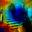
\includegraphics[width=.09\textwidth]{fig/gradient/fig/fig_cam/cosine/gradcampp/4862.JPEG} &
         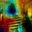
\includegraphics[width=.09\textwidth]{fig/gradient/fig/fig_cam/baseline/scorecam/4862.JPEG} &
         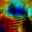
\includegraphics[width=.09\textwidth]{fig/gradient/fig/fig_cam/cosine/scorecam/4862.JPEG} &
         \includegraphics[width=.09\textwidth]{fig/gradient/fig/fig_cam/baseline/ablationcam/4862.JPEG} &
         \includegraphics[width=.09\textwidth]{fig/gradient/fig/fig_cam/cosine/ablationcam/4862.JPEG} \\
    
        {\rotatebox{90}{\tiny \Th{Girl}}} &
        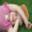
\includegraphics[width=.09\textwidth]{fig/gradient/fig/fig_cam/original/2641.JPEG} &
        \includegraphics[width=.09\textwidth]{fig/gradient/fig/fig_cam/baseline/gradcam/2641.JPEG} &
        \includegraphics[width=.09\textwidth]{fig/gradient/fig/fig_cam/cosine/gradcam/2641.JPEG} &
        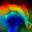
\includegraphics[width=.09\textwidth]{fig/gradient/fig/fig_cam/baseline/gradcampp/2641.JPEG} &
        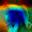
\includegraphics[width=.09\textwidth]{fig/gradient/fig/fig_cam/cosine/gradcampp/2641.JPEG} &
        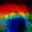
\includegraphics[width=.09\textwidth]{fig/gradient/fig/fig_cam/baseline/scorecam/2641.JPEG} &
        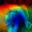
\includegraphics[width=.09\textwidth]{fig/gradient/fig/fig_cam/cosine/scorecam/2641.JPEG} &
        \includegraphics[width=.09\textwidth]{fig/gradient/fig/fig_cam/baseline/ablationcam/2641.JPEG} &
        \includegraphics[width=.09\textwidth]{fig/gradient/fig/fig_cam/cosine/ablationcam/2641.JPEG} \\
    
        {\rotatebox{90}{\tiny \Th{Woman}}} &
        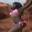
\includegraphics[width=.09\textwidth]{fig/gradient/fig/fig_cam/original/5257.JPEG} &
        \includegraphics[width=.09\textwidth]{fig/gradient/fig/fig_cam/baseline/gradcam/5257.JPEG} &
        \includegraphics[width=.09\textwidth]{fig/gradient/fig/fig_cam/cosine/gradcam/5257.JPEG} &
        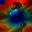
\includegraphics[width=.09\textwidth]{fig/gradient/fig/fig_cam/baseline/gradcampp/5257.JPEG} &
        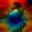
\includegraphics[width=.09\textwidth]{fig/gradient/fig/fig_cam/cosine/gradcampp/5257.JPEG} &
        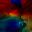
\includegraphics[width=.09\textwidth]{fig/gradient/fig/fig_cam/baseline/scorecam/5257.JPEG} &
        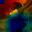
\includegraphics[width=.09\textwidth]{fig/gradient/fig/fig_cam/cosine/scorecam/5257.JPEG} &
        \includegraphics[width=.09\textwidth]{fig/gradient/fig/fig_cam/baseline/ablationcam/5257.JPEG} &
        \includegraphics[width=.09\textwidth]{fig/gradient/fig/fig_cam/cosine/ablationcam/5257.JPEG}\\
    
        {\rotatebox{90}{\tiny \Th{Lobster}}} &
        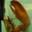
\includegraphics[width=.09\textwidth]{fig/gradient/fig/fig_cam/original/5160.JPEG} &
        \includegraphics[width=.09\textwidth]{fig/gradient/fig/fig_cam/baseline/gradcam/5160.JPEG} &
        \includegraphics[width=.09\textwidth]{fig/gradient/fig/fig_cam/cosine/gradcam/5160.JPEG} &
        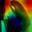
\includegraphics[width=.09\textwidth]{fig/gradient/fig/fig_cam/baseline/gradcampp/5160.JPEG} &
        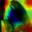
\includegraphics[width=.09\textwidth]{fig/gradient/fig/fig_cam/cosine/gradcampp/5160.JPEG} &
        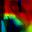
\includegraphics[width=.09\textwidth]{fig/gradient/fig/fig_cam/baseline/scorecam/5160.JPEG} &
        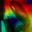
\includegraphics[width=.09\textwidth]{fig/gradient/fig/fig_cam/cosine/scorecam/5160.JPEG} &
        \includegraphics[width=.09\textwidth]{fig/gradient/fig/fig_cam/baseline/ablationcam/5160.JPEG} &
        \includegraphics[width=.09\textwidth]{fig/gradient/fig/fig_cam/cosine/ablationcam/5160.JPEG} \\
    
        {\rotatebox{90}{\tiny \Th{Couch}}} &
        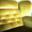
\includegraphics[width=.09\textwidth]{fig/gradient/fig/fig_cam/original/2043.JPEG} &
        \includegraphics[width=.09\textwidth]{fig/gradient/fig/fig_cam/baseline/gradcam/2043.JPEG} &
        \includegraphics[width=.09\textwidth]{fig/gradient/fig/fig_cam/cosine/gradcam/2043.JPEG} &
        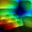
\includegraphics[width=.09\textwidth]{fig/gradient/fig/fig_cam/baseline/gradcampp/2043.JPEG} &
        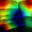
\includegraphics[width=.09\textwidth]{fig/gradient/fig/fig_cam/cosine/gradcampp/2043.JPEG} &
        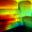
\includegraphics[width=.09\textwidth]{fig/gradient/fig/fig_cam/baseline/scorecam/2043.JPEG} &
        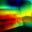
\includegraphics[width=.09\textwidth]{fig/gradient/fig/fig_cam/cosine/scorecam/2043.JPEG} &
        \includegraphics[width=.09\textwidth]{fig/gradient/fig/fig_cam/baseline/ablationcam/2043.JPEG} &
        \includegraphics[width=.09\textwidth]{fig/gradient/fig/fig_cam/cosine/ablationcam/2043.JPEG} \\
    \end{tabular}
%}
    %\vspace{3pt}
    %\caption{\textbf{Saliency map comparison} of standard \vs our training using different CAM-based methods on CIFAR-100 examples.}
    %\label{fig:salient}
    %\end{figure}
    \end{center}
    
\end{frame}

%--------------------------------------------------------------------------------------------------
\begin{frame}[t]
    \frametitle{Results}
    \framesubtitle{Quantitative Experiments}
    \small \textbf{Recognition Metrics}
    \footnotesize
    \begin{center}
        \begin{tabular}{lcccccc}\\\toprule
    \mc{7}{\Th{\textbf{Recognition Metrics}}}\\\midrule
    \Th{Model}&\Th{Error}& &\Th{$\lambda$}&\Th{Acc}$\uparrow$& &\\\midrule
    \mr{2}{\Th{ResNet-18}}&-& &-&\Th{\textbf{73.42}}& &\\
     &\Th{Cosine}& &$7.5\times10^{-3}$&\Th{72.86}& &\\\midrule
     
    \mr{2}{\Th{MobileNet-V2}}&-& &-&\Th{59.43}&\\
     &\Th{Cosine}&  &$1\times10^{-3}$&\Th{\textbf{62.36}}&\\\midrule
\end{tabular}    
    \end{center}\pause
    Recognition properties are maintained.

\end{frame}
%--------------------------------------------------------------------------------------------------
\begin{frame}[t]
    \frametitle{Results}
    \framesubtitle{Quantitative Experiments}
    \small \textbf{Interpretability metrics}
    \footnotesize
    \begin{center}
        \begin{table}[H]
    \centering
    \tiny
    \setlength{\tabcolsep}{2pt}
    %\renewcommand{\arraystretch}{0.8}
    \begin{tabular}{lcccccclcccccc}\\\toprule  
        \mc{14}{\Th{\textbf{Interpretable Recognition Metrics}}}\\\midrule    
        \mc{7}{\Th{ResNet-18}}&\mc{7}{\Th{MobileNet-V2}}\\\midrule
        \Th{Method}&\Th{Error}&\Th{AD$\downarrow$}&\Th{AG$\uparrow$}&\Th{AI$\uparrow$}&\Th{Ins$\uparrow$}&\Th{Del$\downarrow$}&
        \Th{Method}&\Th{Error}&\Th{AD$\downarrow$}&\Th{AG$\uparrow$}&\Th{AI$\uparrow$}&\Th{Ins$\uparrow$}&\Th{Del$\downarrow$}\\\hline
        \mr{2}{\Th{Grad-CAM}}&-&30.16&15.23&29.99&58.47&\textbf{17.47}&\mr{2}{\Th{Grad-CAM}}&-&44.64&6.57&25.62&44.64&\textbf{14.34}\\
         &\Th{Cosine}&\textbf{28.09}&\textbf{16.19}&\textbf{31.53}&\textbf{58.76}&17.57&&\Th{Cosine}&\textbf{40.89}&\textbf{7.31}&\textbf{27.08}&\textbf{45.57}&15.20\\\hline
        \mr{2}{\Th{Grad-CAM++}}&-&31.40&14.17&28.47&58.61&\textbf{17.05}&\mr{2}{\Th{Grad-CAM++}}&-&45.98&6.12&24.10&44.72&\textbf{14.76}\\
          &\Th{Cosine}&\textbf{29.78}&\textbf{15.07}&\textbf{29.60}&\textbf{58.90}&17.22&&\Th{Cosine}&\textbf{40.76}&\textbf{6.85}&\textbf{26.46}&\textbf{45.51}&14.92\\\hline
        \mr{2}{\Th{Score-CAM}}&-&26.49&18.62&33.84&58.42&\textbf{18.31}&\mr{2}{\Th{Score-CAM}}&-&40.55&7.85&28.57&45.62&\textbf{14.52}\\
          &\Th{Cosine}&\textbf{24.82}&\textbf{19.49}&\textbf{35.51}&\textbf{59.11}&18.34&&\Th{Cosine}&\textbf{36.34}&\textbf{9.09}&\textbf{30.50}&\textbf{46.35}&14.72\\\hline
        \mr{2}{\Th{Ablation-CAM}}&-&31.96&14.02&28.33&58.36&\textbf{17.14}&\mr{2}{\Th{Ablation-CAM}}&-&45.15&6.38&25.32&44.62&\textbf{15.03}\\
         &\Th{Cosine}&\textbf{29.90}&\textbf{15.03}&\textbf{29.61}&\textbf{58.70}&17.37&&\Th{Cosine}&\textbf{41.13}&\textbf{7.03}&\textbf{26.10}&\textbf{45.38}&15.12\\\hline
        \mr{2}{\Th{Axiom-CAM}}&-&30.16&15.23&29.98&58.47&\textbf{17.47}&\mr{2}{\Th{Axiom-CAM}}&-&44.65&6.57&25.62&44.64&15.27\\
          &\Th{Cosine}&\textbf{28.09}&\textbf{16.20}&\textbf{31.53}&\textbf{58.76}&17.57&&\Th{Cosine}&\textbf{40.89}&\textbf{7.31}&\textbf{27.08}&\textbf{45.57}&\textbf{15.20}\\\bottomrule
    \end{tabular}
\end{table}
    
    \end{center}
    \pause
    Interpretable properties are enhanced. Deletion still poses an issue.
\end{frame}
\subsection*{Conclusions}
%--------------------------------------------------------------------------------------------------
\begin{frame}
    \frametitle{Conclusions}
    \small
    \begin{itemize}
        \item Denoising CNN gradients improve interpretability properties, maintining recognition.
        \item Negative gradients contribute to stability during training.
        \item Resolution matters: small inputs require shallow layer targeting. 
        \item Published in VISAPP 2024.
    \end{itemize}
    
\end{frame}